\documentclass[11pt, tikz]{standalone}
\usepackage[T1]{fontenc}
\usepackage[utf8]{inputenc}
%\usepackage{textcomp}
%\renewcommand{\ttdefault}{lmtt} % 
\usepackage{amsmath}
\usepackage{amssymb}
\usepackage{mathtools}
\usepackage{commath}
\usetikzlibrary{arrows.meta, decorations.pathmorphing, positioning, calc}
\usepackage{xcolor}

\usepackage{mwe,tikz}
\usepackage[percent]{overpic}
\pagestyle{empty}

\begin{document}\sffamily
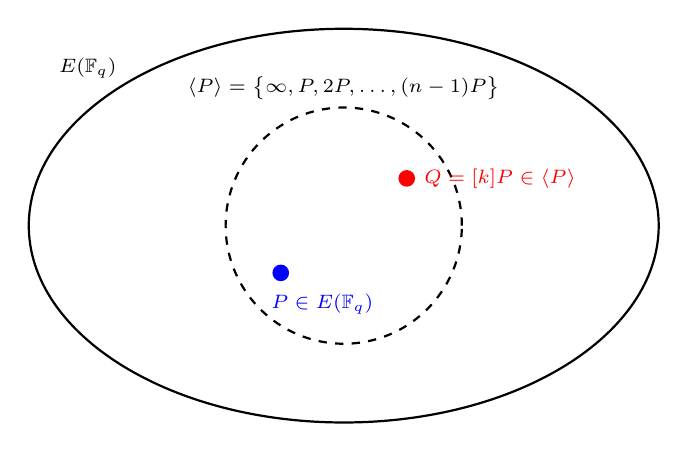
\begin{tikzpicture}
	% Draw the large set for E(F_q)
	\draw[thick] (0,0) ellipse (4 and 2.5);
	\node at (-3.25,2) {\scriptsize  $E(\mathbb{F}_q)$};
	
	% Draw the subset for <P>
	\draw[thick, dashed] (0,0) circle (1.5);
	\node at (0,1.75) {\scriptsize $\langle P \rangle=\set{\infty, P, 2P, \dots, (n-1)P}$};
	
	% Draw a specific point Q
	\fill[red] (0.8,0.6) circle (3pt);
	\node[red, anchor=west] at (0.9,0.6) {\scriptsize  $Q = [k]P\in\langle P\rangle$};
	
	% Add generator P for clarity
	\fill[blue] (-0.8,-0.6) circle (3pt);
	\node[blue, anchor=east] at (.5,-1) {\scriptsize  $P\in E(\mathbb{F}_q)$};
	
	% Add a label for the cyclic subgroup
%	\node[anchor=north] at (0,-1.8) {\large Cyclic subgroup $\langle P \rangle \leq E(\mathbb{F}_q)$};
\end{tikzpicture}
\end{document}
